\documentclass[a4paper, 11pt, oneside]{book}
\usepackage{fontspec}
\usepackage{lmodern}
\usepackage[czech]{babel}
\usepackage{csquotes}
\usepackage{url}
\usepackage{todonotes}
\usepackage{xunicode}
\usepackage{graphicx}
\graphicspath{ {imgs/} }

\usepackage[
   backend=biber
  ,style=iso-authoryear
  ,sortlocale=cs_CZ
  ,autocite=footnote
  ,maxnames=2
  ,minnames=1
  ,urldate=long
  ,spacecolon=false
  ]
  {biblatex}


\addbibresource{bibliografie.bib}

\newcommand{\td}[2][]{
	{\todo[size=\footnotesize]{#2}}
}

\author{edík}
\title{Magi}

\newcommand\ex{\textsf}

\begin{document}

	\maketitle

	\newpage

	\tableofcontents

	\newpage

	\part{Teoretické pojednání}

	\chapter{Princetonský WordNet} % (fold)
	\label{cha:princeton_wn}
	
		Princetonský WordNet je prvním wordnet vůbec. Vznikal na univerzite v Princetonu pod G. A. Millerem od poloviny 80. let 20. století. Vzhledem k tomu, že byl prvním wordnetem, bylo k němu referováno jako k WordNetu, bez přívlastku. Ačkoliv tento stav v podstatě přetrvává dodnes, oproti době jeho vzniku se situace změnila, vzniklo několik dalších wordnetů a nastala tudíž potřeba je rozlišit. V anglickém prostředí se obvykle pojmem WordNet míní ten princetonský a všechny ostatní wordnety mají přívlastek. Příkladem nechť je Balkanet či Eurowordnet. Ačkoliv v mezinárodním prostředí je obvyklé přívlastek \uv{princetonský} používat, bude tato práce pracovat s následujícím rozlišením:\td{a samozrejme bych to actually mohl dodrzovat, tohle jsem si vymyslel az po napsani tehle kapitoly, lol}

		\begin{itemize}
			\item \textit{WordNet} (ve významu princetonský WordNet)
			\item \textit{wordnet} (ve významu obecné sémantické sítě založené ideou, obsahově či strukturálně na WordNetu)
			\item konkrétní wordnety, např. \textit{Balkanet}
		\end{itemize}

		\section{Motivace vzniku}
			Od počátků snah o zpracování přirozeného jazyka (NLP, natural language processing) bylo nutné poskytnout programu data o lexiku ve zpracovávaném textu, ať už ona data byla jakákoliv. Kupříkladu pro překlad se mělo za to, že stačí ekvivalentní dvojice ve zdrojovém a cílovém jazyce, později se přidal kontext v případě statistického strojového překladu spolu s dalšími informacemi, jako je například slovní druh. Tradičně se lexikální materiál ukládá způsobem nikoliv diametrálně odlišným od papírových slovníků určených pro lidské uživatele. Ty obvykle obsahují abecenedně (či podle jiného indexu \td{cit?}) seřazené jednotlivé záznamy s potřebnými informacemi o slovech, z nichž pak program může čerpat při zpracování textu.

			Jak uvádí \textcite{pala2013vceska}, uspořádání lexikálního materiálu v takovéto formě je sice vhodné pro člověka, ale nikoliv pro strojové zpracování, a to z několika důvodů. Kromě toho, že vyhledávání v abecedním seznamu je relativně pomalé \td{nejaka citace?, dohledat neco, jak takovy slovniky byly ulozeny...}, struktura tradičního slovníku kvůli onomu abecednímu řazení inherentně vzdaluje slova, jež člověk chápe jako nějakým způsobem blízká. Tato blízkost může vyplývat ze vztahu volné synonymie, antonymie, podřazenosti, nadřazenosti, etc. Pokud si tedy například uživatel výkladového slovníku nepříliš obeznámený s daným jazykem vyhledá určité heslo, dozví se sice pravděpodobně jeho význam, ale nebude schopen své znalosti prohlubovat dále zjištěním, kupříkladu jaké je slovo odpovídá opačnému významu.

			Dalším všeobecným problémem při využití tradičních slovníků k počítačovému zpracování jazyka je fakt, že lexikografové předpokládají u uživatele slovníku značné encyklopedické znalosti. Zařazují tak do slovníku jen informace dle jejich názoru důležité pro rozlišení (differentia specifica) a zařazující do kontextu či přiřazující k určité nadřazené třídě objektů (genus proximum). Vyhledá-li si tedy člověk ve Slovníku spisovného jazyka českého\td{citace} heslo \ex{vlk}, zjistí následující:

			\ex{\textbf{vlk: } psovitá šelma šedě (n. šedožlutě) zbarvená, žijící v Evropě, Asii a v Sev. Americe}

			Definice a priori předpokládá, že uživatel je obeznámen s tím, co je \ex{šelma} a co je \ex{pes}. Pokud takovou znalostí neslyne (což je vcelku představitelné například u cizince), je nucen si tato slova ve slovníku najít a podívat se na jejich definice (pomiňme nyní netriviální úkol převést slovo \ex{psovitá} na základní tvar \ex{pes}). Pokud nerozumí definicím ani nadřazených slov, musí pokračovat v hierarchii dále a dále. 

			Z uvedeného případu plyne, že jakkoliv je možné správným vyhledáváním hyperonym\footnote{nadřazené slovo} dospět k tomu, že \ex{vlk} je konkrétní entita našeho vesmíru, živá bytost o čtyřech končetinách, savec nějakým způsobem přibuzný se psovi, má šedou srst etc., je takový proces dosti komplikovaný. Případ s cizincem se sice nemusí zdát zcela relevantní, protože se dá předpokladat, že daný člověk má, byť v jiném jazyce, stejné základní znalosti předpokládané lexikografy jako člověk český. Situace je však dramaticky jiná u počítače. Na rozdíl od člověka totiž počítač nemá žádné předchozí znalosti, tudíž musí projít celým procesem popsaným výše, aby byl schopen kupříkladu určit, že \ex{vlk} může umřít (ježto je živá bytost). Protože však tradiční slovníky typu SSJČ byly vytvářené pro papírové médium, neobsahují žádné propojení ve stylu \textit{toto je odkaz na hyperonymum}, a počítač tudíž jen těžko může zjišťovat, na které vlastně slovo se to má podívat, aby se dobral podstaty pojmu \ex{vlk}.

			\subsection{Strojově čitelné slovníky}

				V zájmu automatizace vyhledávání ve slovníku vznikaly tzv. strojově čitelné slovníky\footnote{machine readable dictionary}, což je pojem souhrnně označující lexikální databáze. Podle množství informací, které taková databáze obsahuje, pak lze tyto dělit na slovníky, taxonomie a ontologie. Je evidentní, že obyčejný slovník neobsahuje oproti tradičnímu papírovému slovníku navíc žádné metainformace, takže je počítač při jeho užívání v podstatě omezen na elektronický listovač \parencite{miller1990introduction}. 

				Míra, jakou se strojově čitelný slovník odliší od pouhé zdigitalizované formu papírového slovníku a přiblíží se k pokročilé lexikální databázi, lze vyjádřit v několika stupních. V případě, že slovník má jednotlivé významy\td{nejakej link, kde budou významy/senses vysvetleny} uspořádány v hierarchii dle nadřazenosti--podřazenosti, lze jej označit za taxonomii, tedy systém s hlubší strukturou než pouze abecedním řazením hesel. 

				Dalším stupněm už je skutečná lexikální databáze, která má jednotlivé významy propojeny rozličnými vztahy, počínaje onou základní hyperonymií a hyponymií a pokračuje kupříkladu vztahy meronymie\footnote{vztah \textit{je částí}, tedy např. \ex{dveře} je meronymem \ex{trolejbusu}} či antonymie\footnote{protikladu}. Kromě vztahů mezi významy bude taková lexikální databáze obsahovat zřejmě i další informace, tedy nějaké kategorie slov, jejich popis, etc. Databáze tak popsaných významů propojených sémantickými vztahy může být nazývána ontologií.\parencite{garshoi2004metadata}

			\subsection{Od slovníků k WordNetu}

				Výše uvedená opozice papírového slovníku a ontologie ilustruje rozdíly tradičního slovníku a počítačově zpracovatelné lexikální databáze. Už ze samotného významu takové databáze je evidentní jeden klíčový rozdíl -- tradiční slovníky, jsouce řazené abecedně, od sebe oddalují některá hesla, jež by bylo vhodné mít pohromadě \parencite{pala2013vceska}. Příkladem budiž \ex{kostra} a její části, např. \ex{lebka}. V SSČ\footnote{Slovník spisovné češtiny} i SSJČ se u \ex{lebky} uvádí, že jde o \ex{kostru hlavy}. Lze tedy s jistou rezervou tvrdit, že heslo obsahuje své holonymum\footnote{vztah opačný k meronymii; tedy např. \ex{dům} je holonymem pro \ex{okno}, \ex{dveře}, \ex{práh} etc.}, opačně to však již nefunguje. Z celkem evidentních důvodů nejsou u hesla \ex{kostra} uvedeny všechny její části. Tento příklad příhodně ukazuje i jistou nesystémovost tradičních slovníků, která je pro počítačové zpracování fatální. % a pak ty slovni druhy, vole!

				Naznačeny tedy byly vlastnosti, jež by databáze významů měla oproti tradičnímu slovníku mít, aby byla použitelná pro počítačové zpracování přirozeného jazyka. Především jde o systémovost vztahů. Hypero/hyponymie je vztah oboustranný, tudíž by mělo být možné se stejnou cestou dostat od nadřazeného slova k podřazenému a naopak. Dále jsou podstatné pojmenované sémantické vztahy mezi slovy. Díky nim je totiž možno jednoznačně určit, které slovo (či slova) je v takové databázi konkrétnímu slovu nadřazené, které je jeho specifikací, označením jeho částí, etc. 

				S touto myšlenkou vznikl WordNet - lexikální síť provázaná sémantickými vztahy, která by dle poznatků psycholingvistiky odrážela uspořádání lexikálního materiálu v lidském mozku (o tom v dalších kapitolách\td{ref}). \parencite{pala2013vceska} Zde by bylo na místě poznamenat, že ačkoliv se tak z odstavců výše může čtenáři jevit a i všeobecně je to často tvrzeno, WordNet není ontologií v pravém slova smyslu, protože něco něco.. \url{https://en.wikipedia.org/wiki/WordNet#WordNet_as_a_lexical_ontology} \td{a tady tomu vubec nerozumim, ale prijde mi to relevantni }

				% nekde u psycholingvistiky to s tim kanarkem, zpivanim a mitim kuze a tak

		\section{K vlivu psycholingvistiky na organizaci WordNetu}
		\label{cha:psycho}

			G. A. Miller, který je tvůrcem WordNetu, se po spolupráci s Chomskym na základních kapitolách jeho \textit{Handbook of Mathematical Psychology}\td{cit}, která se věnuje spíše syntaktickému popisu jazyka, se zaměřil společně s Johnsonem-Lairdem na výzkum, jakým způsobem je lexikální materiál uložen v lidském mozku. Tento přístup je označován jako psycholingvistika a jeho počátky jsou spojeny s průzkumem asociací a budování modelu mentálního slovníku člověka. Výchozí myšlenka, jež se odráží i ve způsobu organizace WordNetu, spočívá v tom, že slovní zásoba není organizována abecedně, jako tomu je v tradičních slovnících, ale spíše konceptuálně. 

			Jednou z otázek tohoto směru bylo, jakým způsobem je organizována paměť. Aby člověk byl schopen určit pravdivostní hodnotu výroku \ex{Kanárek může létat}, musí použít svou dlouhodobou pamět. Její organizace je pak možná (minimálně) dvěma způsoby. První, redundantní, by vypadal tak, že by u každého ptáka bylo uloženo, že je schopen létat. Druhý, již na první pohled výrazně méně náročný na úložný prostor, by příznak schopnosti létat měl uložený pouze u kategorie \ex{pták}. V případě, že by bylo třeba zjistit, zda kanárek léta, by bylo nutno pak zapojit inferenční proces ve stylu \textit{kanárek je pták, tudíž může létat}. \parencite{collins1969retrieval}

			Jak \textcite{collins1969retrieval} dále uvádí, lze předpokládat, že v případě prvního způsobu organizace paměti by člověk mohl kteroukoliv informaci o příznacích (vlastnostech) z paměti vyvolat za konstantní čas. Naproti tomu v případě způsobu druhého by extrakce příznaku z významu v hierarchii položeného výše měla trvat delší čas než extrakce příznaku přítomného přímo u významu, jenž je objektem věty. Důvodem by měla být nutnost zapojení inferenčního procesu.

			Pokus, kterým podpořili \textcite{collins1969retrieval} druhý, neredundantní, způsob organizace paměti, spočíval v tom, že testovací subjekty, dobrovolníci z řad zaměstnanců společnosti Bolt Beranek and Newman, měly určovat, zda je výrok pravdivý, či nepravdivý. Měli tak činit co nejpřesněji a v co nejkratším čase, přičemž byla měřena rychlost jejich reakce. Ukázalo se, reakční doba při určování pravdivosti výroku \ex{Kanárek umí létat}\footnote{angl. \ex{A canary can sing}} je delší než při určování pravdivosti výroku \ex{Kanárek umí zpívat}\footnote{angl. \ex{A canary can sing}} a ještě delší při určování výroku \ex{Kanárek má kůži}\footnote{angl. \ex{A canary has skin}}. Důvodem pro tyto progresivní prodlevy podle nich právě byla zvětšující se vzdálenost od významu \ex{kanárka} ke významu, u něhož byl uložen příslušný příznak, tedy \ex{umí zpívat}, \ex{umí létat}, resp. \ex{má kůži}. Příznak \ex{umí zpívat} totiž je pravděpodobně uložen přímo u \ex{kanárka}, jelikož jej odlišuje od ostatních ptáků, zatímco příznak \ex{umí létat} je obecným znakem ptáků, tudíž je uložen u významu \ex{pták}. V poslední řadě pak příznak \ex{má kůži} bude patrně uložen u významu \ex{zvíře}, který je oněch tří v hierarchii nejvýše, a ze všech tudíž od kanárka nejdále.

			Jelikož WordNet G. A. Millera je založen na podobném principu\td{cit}, lze říci jistým způsobem odráží organizaci lexika v lidském mozku.

		

		\section{Organizace WordNetu}

			Ve WordNetu lze nalézt informace autosémantikách, tedy substantivech, adjektivech, slovesech a příslovcích \parencite{vossen1998introduction}. Synsémantika (např. předložky, spojky etc.) nebyla zahrnuta, jelikož se zdá, že jsou uložena odděleně od slov plnovýznamových. 

			% \subsection{Psycholingvistická podpora organizace WordNetu}

			Teorii, že jsou funkční slova uchovávána jako součást syntaktikonu, podpořil kupříkladu \textcite{garrett1982production} při svém pozorování afatických pacientů. Stejně jako je výběr slovních druhů zastoupených ve WordNetu podložen předpokládanou organizací lexikálního materiálu v lidském mozku, je i samotné seskupování lexika podle slovních druhů (na rozdíl od abecedního řazení v tradičních slovnících) podloženo výsledky průzkumu dalšího aspektu jeho organizace. \textcite{fillenbaum1965grammatical} provedli asociační test na anglicky mluvících subjektech, kteří měli za úkol uvést první slovo, které je napadne v kontextu dobře známých slov, která jim byla předkládána. Tato slova náležela k různým slovním druhům a ukázalo se, že ve většině případů náleží asociované slovo ke stejnému slovnímu druhu jako slovo, které asociaci vyvolalo. Substantiva vyvolala asociaci na substantivum v 79 \% případů, adjektiva v 65 \% případů a slovesa v 43 \% případů. Ačkoliv není zřejmé, jak je znalost o slovním druhu určitého slova získávána, lze z uvedených dat předpokládat, že slovní druh je vskutku primární organizační vlastností lexikálního materiálu v lidském mozku a informace o něm je snadno dostupná (alespoň intuitivně). 

			Seskupování konceptů podle slovního druhu a zřejmě navzdory snaze o ekonomii ukládání informací, kterou se lidský mozek vyznačuje, zprostředkovaně vede k jisté redundantnosti systému. Existuje totiž mnoho slov (zvláště např. v angličtině), která zastupují jak substantivum, tak verbum (např. angl. \ex{show}, popř. české \ex{stát}). Jelikož spolu taková slova kromě formy nemají příliš mnoho společného a náleží do odlišných konceptů, jsou takové výrazy uloženy zcela nezávisle a bez propojení sémantickými vztahy. Tento koncept podporuje i fakt, že se evidentně chovají zcela odlišně v rovině syntaktické.\textcite{miller1990introduction} Co se provázání vztahy týče, dá se předpokládat, že člověk je schopen se dobrat k různým významům stejné formy, avšak zřejmě nepůjde o sémantický vztah, ale spíše asociaci přes podobnost formy. WordNet homonymii zohledňuje vztahem derivačně příbuzné formy\footnote{derivationally related form}, který je definován jako spojení slov (tedy nikoliv konceptů) náležících do různých syntaktických kategorií a majících (blíže nedefinovanou) sémantickou příbuznost\td{cit: https://wordnet.princeton.edu/wordnet/man/wngloss.7WN.html}. Principiálně jde tedy o vztah zcela odlišný od čiště sémantických vztahů propojujících celé koncepty.

			Motivací pro tvorbu WordNetu je, jak bylo popsáno v předchozích kapitolách, mít k disposici informace o slovní zásobě, již bude možno použít k inferenčnímu vyvozování závěrů (získávání informací) o slovech, a to strojově, což znamená bez nutnosti mít jakékoliv předchozí encyklopedické znalosti, které má obvykle uživatel tradičního slovníku k disposici. Jednotlivé položky slovní zásoby tedy musí být propojeny vztahy, z nichž bude obecně zřejmé, jakou informaci inferenční stroj získá, přejde-li po onom vztahu k dalšímu slovu. Slovní zásoba je proto ve WordNetu propojena pomocí několika sémantických vztahů, které určují její hierarchizaci a odráží například i vzdálenost konceptů (relevantní kupříkladu pro časovou náročnost vyhodnocení pravdivosti výroku, podr. v kap. \ref{cha:psycho} na straně \pageref{cha:psycho}). Hierarchizaci slovní zásoby ve WordNetu lze naznačit grafem \ref{fig:hierchWN} na straně \pageref{fig:hierchWN} (daco takoveho, ale ne tak krepo nakresleneho). 

			\begin{figure}[h]
				\centering
				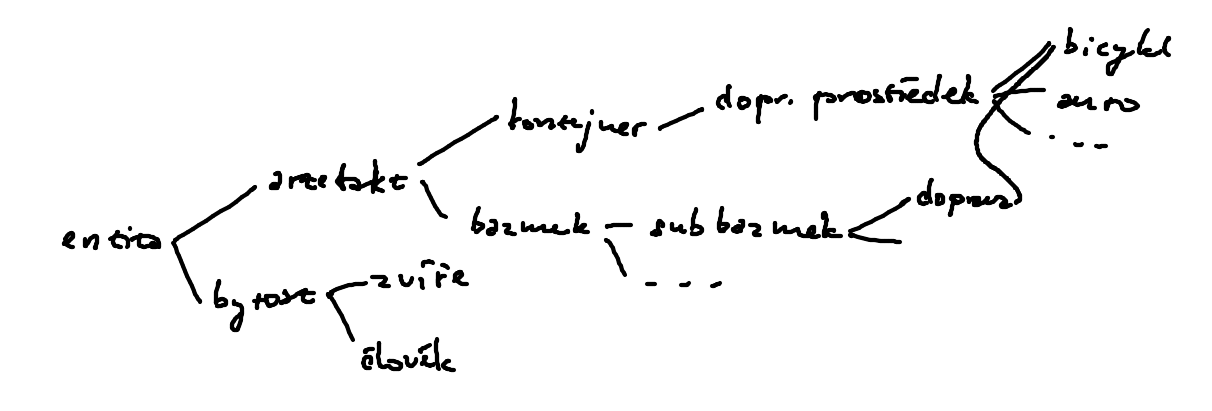
\includegraphics[width=1.0\textwidth]{screenshot_2017-03-31_14-14-36.png}
				\caption{Hierarchizace slovní zásoby ve WordNetu}
				\label{fig:hierchWN}
			\end{figure}

			Hierarchická organizace významů substantiv\footnote{a možná i dalších slovních druhů} ve WordNetu tak, jak byla naznačna na grafu \ref{fig:hierchWN} na straně \pageref{fig:hierchWN}, je podpořena i poznatkem, že lidé jsou schopni velice rychle zpracovávat anaforické a kataforické výrazy a komparativní konstrukce. Například ve větě \ex{Vlastnil pušku, ale z té zbraně se nikdy nevystřelilo.} je každému čtenáři zřejmé, že výraz \ex{ta zbraň} odkazuje k výrazu \ex{puška}.\footnote{Zajímavé je uvažovat o významu této věty při vypuštění deiktického \ex{ta} -- zdá se, že pak už anaforický odkaz k \ex{pušce} nefunguje a z věty se stává jakési nesmyslné spojení dvou výroků -- konkrétního (\ex{Vlastnil pušku} a zcela obecného (a evidentně nepravdivého) \ex{ze zbraně se nikdy nevystřelilo}.} Co se zmíněného zpracovávání komparace týče, lze říci, že nelze porovnávat dvě substantiva, která jsou provázána sémantickým vztahem hyperonymie-hyponymie. Výrok \ex{Puška je bezpečnější než zbraň} je zcela nesmyslný. \parencite{pala2013vceska} % nasledujici je asi uplne blbost: \footnote{Porovnání substantiv svázaných vztahem hyperonymie--hyponymie však je možné v případě, že je vypuštěno \ex{než}; specifičtějšímu ze slov se tím pak přisuzuje rys, jenž u hyperonyma není přítomen, či se rys hyperonyma stupňuje: \ex{bytový dům je takový hezčí panelák} či \ex{rys je taková divočejší kočka} (lípa je takový vyšší strom, panelák je takový vyšší dům, ...)}.
		

			

			\subsection{Struktura hesla}

		
		% \section{Historie WordNetu}

		% 	- WordNet was created in the Cognitive Science Laboratory of Princeton University under the direction of psychology professor George Armitage Miller starting in 1985
		% 	- been directed in recent years by Christiane Fellbaum
		% 	- George Miller and Christiane Fellbaum were awarded the 2006 Antonio Zampolli Prize
		% 	- As of November 2012 WordNet's latest Online-version is 3.1.

		\section{Sémantické vztahy WordNetu}
		\label{cha:sem-vztahy}

			Jak bylo naznačeno výše, koncept WordNetu je založen na lexikální sémantice, tedy představě, že slovo je kombinací slovní formy a významu, nebo slovního významu. Slovní forma je projevem \uv{fyzickým}, tedy je to vyřčená či napsaná instance významu. Jak je zjevné z přirozeného jazyka, nelze počítat s tím, že by zobrazení významu na formu bylo bijektivní, tedy každý význam byl namapován jedna ku jedné na slovní formu. Mapování je v přirozeném jazyce tzv. více ku více, tedy jedna forma může zastupovat více významů a jeden význam může být vyjádřen více formami. Je velmi časté, že jedna slovní forma zastupuje více významů. Kupříkladu slovní forma \ex{koruna} může zastupovat význam měny, vrcholku stromu, vladařského odznaku, etc. Toto zobrazení se nazývá homonymií\footnote{totožnost formy}. Možný je samozřejmě i opačný případ, kdy více významům slouží k vyjádření jedna slovní forma, což je nazýváno polysémií\footnote{víceznačností}. Příkladem může být forma \ex{kolej}, již lze interpretovat jako referenci k stopě po voze, případně dvojici kolejnic jako vodící dráze pro dopravní prostředky\td{cit. SSJC} a zároveň jako zařízení vysoké školy pro ubytování studentů.\td{cit SSJC}

			\textcite{miller1990introduction} popisují výše naznačené vztahy pomocí takzvané lexikální matice. Ta názorně zobrazuje formy synonymní ($F_1$ a $F_2$) a formy polysémní ($F_2$):

			{\tt tabulka z miller1990introduction pg. 4: http://i.imgur.com/sohtwe5.png}

			\td{tady by jeste slo pokracovat opisovanim dalsi casti toho clanku (miller1990introduction pg 5 >>>)}

			V dalších podkapitolách budou rozebrány podrobněji, nikoliv však vyčerpávajícím způsobem, sémentické vztahy konstituující Wordnet. Jelikož se sémantické vztahy pro jednotlivé slovní druhy liší, bude tato kapitola strukturována primárně právě podle slovních druhů a až sekundárně podle sémantických vztahů.

			% proc musi sem. vztahy byt rozdelene podle PoS: o subst. nelze moc rikat, ze jsou antonymni, etc.., 

			\subsection{Frekvenční distribuce sémantických vztahů ve WordNetu}

				% nejdriv nutno zjistit, jak je to s temi vztahy ruznych slovnich druhu... jinak ta statistika nedava vuebc smysl 

			\subsection{Substantiva}


				\subsubsection{Synonymie}

					Synonymie je centrálním organizačním vztahem pro substantiva ve WordNetu. Na praktických aplikacích je tento jev nejlépe pozorovatelný, jelikož při vyhledání konkrétní formy je uživateli obvykle nabídnut výběr z jednotlivých významů dané formy. Aby byly od sebe významy oné formy odlišitelné, nabídka běžně sestává z výpisu skupin forem (tzv. synsetů, o tom později), přičemž každá skupina náleží k jednomu významu a obsahuje formy danému významu přiřazené. Kupříkladu při vyhledání slova \ex{kolo} tak je uživatel konfrontován s několika skupinami, které obsahují zhruba následující:

					\begin{itemize}
						\item \ex{kolo (1)},
						\item \ex{jízdní kolo (1), bicykl (1), kolo (2)},
						\item \ex{kružnice (1), cívka (1), kolo (3)},
					\end{itemize}

					přičemž čísla (zde) v závorce značí index významu dané formy v daném synsetu. Reprezentace v různých aplikacích a různých wordnetech se liší (standardem bývá číslo významu psát za dvojtečku), koncept však zůstává neměnný. 

					Navzdory zdánilivé jednoduchosti výše uvedeného konceptu je všeobecnou otázkou, jak synonymii pojímat. Striktní teorie (obvykle připisovaná Leibnizovi) praví, že dvě slova jsou synonymní, pokud se jejich záměnou nikdy nezmění pravdivostní hodnota výroku. Lingvistickou interpretací tohoto poněkud matematicko-logického výroku může pak být, že synonymní dvě slova jsou v případě, že se jejich záměnou nikdy neporuší význam (zhruba ona pravdivostní hodnota) a gramatičnost výroku. Je nasnadě, že takto striktně synonymní slova budou pospolu v jazyce těžko přežívat, jelikož je dokázáno, že jazyk tíhne k ekonomičnosti, která by takovým soužitím dvou slov byla hrubě porušena. Pravděpodobně jedinými obecně uznávanými synonymy jsou obvykle dvojice cizího slova a domácího slova, například \ex{internacionální} a \ex{mezinárodní}. S relativně vysokou jistotou lze tvrdit, že jejich záměnou se nikdy pravdivostní hodnota výroku nezmění, stejně tak jako jeho gramatičnost. Stále však zůstává ve hře stylistika, která může být podobnou náhradou narušena (např. z důvodu cílové skupiny čtenářů či stylistické příznakovosti jednoho ze slov (srov. \ex{zajímavý} a \ex{interesantní})). Co se tendence k ekonomičnosti jazyka týče, lze předpokládat, že v těchto případech převládá potřeba synonym k eliminaci opakování určitých slov v textu a tím zajištění jeho stylistické uhlazenosti. 

					Volnější interpretace synonymie také počítá s kontextem. Dvě slova jsou synonymní, jsou-li bez způsobení škod nahraditelná alespoň ve stejném kontextu. Jako příklad mohou posloužit formy \ex{board} a \ex{plank}\td{najit ceske priklady}. V kontextu dřevařství mohou tyto dvě formy pravděpodobně bez problému být nahrazeny jedna za druhou, ovšem v případě, že je forma \ex{board} použita ve významu \ex{comittee}, těžko ji lze nahradit za formu \ex{plank}, neboť by se věta obsahující takové nahrazení stala zcela nesmyslnou.

					Bylo by nanejvýš logické považovat synonymii za vztah diskrétní, tedy že dvě formy buďto synonymní jsou, či nejsou. Z logického hlediska to nepochybně z již uvedeného vyplývá, ovšem lingvisticko-filosofický náhled výcházející z poznatků reálného jazyka se na tuto problematiku poněkud liší. Jak bylo dokázáno, synonymie v striktním slova smyslu je velice vzácná. Její volnější interpretace je značně častější, ale také výrazně vágnější -- kontext, v němž dvě formy synonymní jsou může být velmi široký, či naopak velice úzký. Záměna některých dvojic (obecně n-tic, lze ale předpokládat, že mnoho forem nebude mít dvě další synonymní) může měnit stylistiku a význam výpovědi více či méně, přičemž ony dvě formy stále dle daných kritérií lze považovat za synonymní. Nelze tedy než vyvodit, že synonymie, minimálně z pohledu přirozeného jazyka, je jevem graduálním, a některé formy jsou tak \textit{synonymnější} než jiné.

					Zaměnitelnost forem podporuje ještě jeden koncept, na němž je WordNet postaven, a to fakt, že jednotlivé významy jsou seskupovány podle slovních druhů. Jak již bylo řečeno, tento systém vede k jisté redundantnosti, jelikož zvláště v syntetických\td{check, nekecam?} jazycích, jako je kupříkladu angličtina, lze nalézt mnoho případů, kdy identická slovní forma zastupuje více slovních druhů. Významy, které taková slovní forma zastupuje (napříč slovními druhy), mohou být velice blízké, nikdy však nebudou stejné (nelze říci, že význam slovesa \ex{run}\footnote{běžet} a substantiva \ex{run}\footnote{běh} je identický). Jejich záměnou by se sice nestalo vůbec nic, jelikož čtenář či posluchač textu, v němž taková záměna nastala, by automaticky formu interpretoval ve prospěch správného slovního druhu, avšak pokud by slovní druh byl nějakým způsobem \uv{vynucen} (nechť nyní čtenář pomine úvahy, jakým způsobem lze \uv{vynutit} slovní druh formy), stala by se výpověď zcela negramatickou a nesmyslnou. 

					Seskupování významů podle slovních druhů a seskupování forem dle vztahu synonymie se tedy zdá v případě lexikální databáze určené pro strojové zpracování jako vhodným konceptem. Oproti tradičním slovníkům se totiž počítačově zpracovávaná lexikální databáze nemusí potýkat s problémem lidského faktoru -- jednotlivé synonymické řady je stroj schopen prohledávat, na rozdíl od člověka, velice účině, a nahradí tak v případě, že WordNet používá člověk, neúčinné lidské procházení restříkového obsahu.\td{psano v chvatu, mohlo by se to mozna trochu uhladit...}

					% centralni jednotka WN, davalo by smysl rozlisovat syn. mezi formami a mezi vyznamy, ale pro technickou jednoduchost se to nedela; je to symetricka relace a pokud jsou ji spojeny vyznamy, pak i jejich formy; zamenitelnost - silna: zamenou se nemeni pravdivost vyroku, slabsi: podle kontextu - vyznam se v kontextu zamenou nezmeni (plank × board); z toho plyne nutnost redundance slovnich druhu (show a show nelze zamenit); z log. hlediska diskretni (bud slova syn. jsou ci ne), ale z lingv./fil. hlediska gradient - nektere dvojice jsou syn~ctejsi nez jine- porad je to ale reflexivni; 
				
			% slovesa nemaji meronymii, ale has_a relation -- entailment

			\subsection{Antonymie}

				% tak jaky tam vlastne jsou vztahy? jsou deleny pro PoS, ci nikoliv?
	% chapter princeton_wn (end)

	\chapter{Další wordnety} % (fold)
	\label{cha:dalsi_wordnety}
	
		Podle vzoru princetonského WordNetu začaly postupně vznikat i další sémantické sítě založené na stejném konceptu. Tyto sémantické sítě se samozřejmě svou strukturou do větší či menší míry liší\td{nakou kurva citaci}, hlavním kritériem pro to, aby mohly být považovány za wordnet, je to, aby obsahovaly synsety a hyponyma\td{http://globalwordnet.org/wordnets-in-the-world/}. % Jelikož se tato práce bude primárně zabývat wordnetem českým, bude pro srovnání uvádět dva hlavní evropské vícejazyčené wordnety, a to Eurowordnet a Balkanet. 

		\section{EuroWordNet} % (fold)
		\label{sec:eurowordnet}
		
		% section eurowordnet (end)
		

		\section{BalkaNet} % (fold)
		\label{sec:balkanet}
		
		% section balkanet (end)

	% chapter dalsi_wordnety (end)




	% \begin{spacing}{1.05}
	\printbibliography[title={Seznam literatury}]
	% \end{spacing}

	\addcontentsline{toc}{chapter}{Seznam literatury}

\end{document}